%%=============================================================================
%% Performantietest
%%=============================================================================

\chapter{Performantie test}
\label{ch:performantietest}

In dit hoofdstuk worden de resultaten besproken van de uitgevoerde performantietests.

De performantie van beide systemen werden op twee manieren getest:
Eerst werd de benodigde tijd gemeten voor het uitvoeren van het 'vagrant up'-commando. 'vagrant up' installeerde en configureerde het besturingssysteem, de applicaties en de containers vanaf nul.

Vervolgens werd de benodigde tijd gemeten bij het uitvoeren van het 'vagrant provision'-commando. Hierbij waren het besturingssysteem en de applicaties al geïnstalleerd en geconfigureerd, en moesten alleen de containers nog tot stand gebracht worden. Om de internetsnelheid als factor te schrappen, waren de Docker Images ook al gedownload.

Daarnaast werd 'time' als prefix aan het commando toegevoegd. Hierdoor werd er op het einde van de commando's de tijd getoond die nodig was voor het uitvoeren.

Vervolgens werden beide commando's vijftien keer uitgevoerd op beide opstellingen. Hierdoor werd de invloed van outliers vermindert. Outliers zijn observatiepunten die ver van andere punten verwijdert liggen.

Ten slotte werden deze resultaten genoteerd in een tabel in Rstudio. Zodanig dat deze resultaten konden worden gebruikt om het gemiddelde, de variantie en standaarddeviatie te gereken. Alsook voor het generen van een scatterplot en boxplot.

\section{CentOS 7.4}

\subsection{Performantie installatie}
Hieronder kan men de eerste resultaten zien van het 'time vagrant up'-commando voor de CentOS-opstelling.

%% plot
\begin{center}
	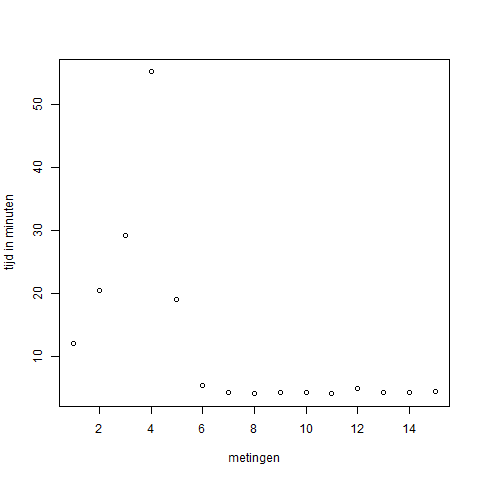
\includegraphics[scale=0.5]{img/centosplotfull.png}
\end{center}

%% boxplot
\begin{center}
	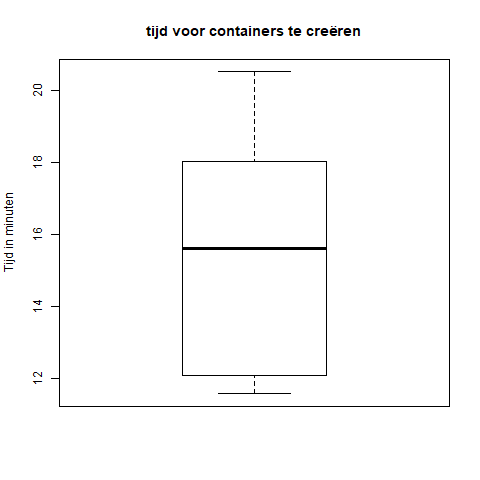
\includegraphics[scale=0.5]{img/centosboxplotfull.png}
\end{center}

%% gemiddelde
$\mu = 12.06457$

%% variantie
$\sigma^2 = 203.7204$

%% standaarddeviatie
$\sigma = 14.27307$

De gemiddelde benodigde tijd voor het commando bij de CentOS-opstelling was laag en vrijwel stabiel, met maar een paar outliers. De reden voor deze outliers kwam omdat deze metingen genomen waren in een omgeving met een slechtere internetverbinding.

Dit was dus de grootste bottleneck voor deze opstelling. De impact hiervan op de installatie was in dit geval groot, zoals te zien valt aan de hoge variatie en standaarddeviatie.

Maar, in het algemeen valt was de performantie van de CentOS-opstelling goed te noemen.

\subsection{Performantie containers}
Vervolgens kan men hier de resultaten zien voor elke keer dat het 'time vagrant provision'-commando werd uitgevoerd op de CentOS-opstelling. Deze keer uitgedrukt in seconden.

Bij deze resultaten moest het Operating System niet meer geïnstalleerd worden en ook de Docker Image moeten niet meer gedownload worden. Er werd alleen gekeken hoelang de Docker Daemon nodig had om de orders te interpreteren en de container tot staand te brengen.

%% plot
\begin{center}
	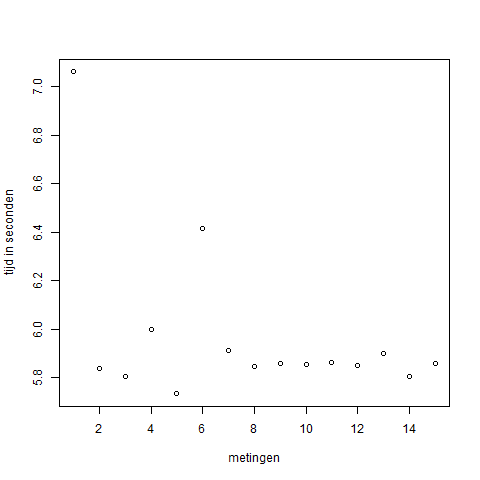
\includegraphics[scale=0.5]{img/centosplotprovision.png}
\end{center}

%% boxplot
\begin{center}
	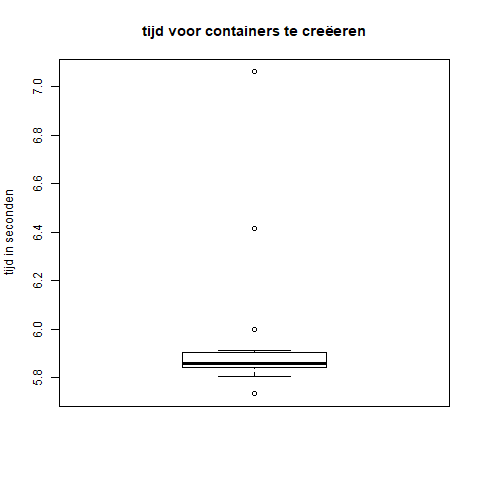
\includegraphics[scale=0.5]{img/centosboxplotprovision.png}
\end{center}

%% gemiddelde
$\mu = 5.972333$

%% variantie
$\sigma^2 = 0.1150491$

%% standaarddeviatie
$\sigma = 0.3391889$

De installatie van alleen de container ging vlot, met een stabielere gemiddelde tijd, en een kleinere variantie en standaarddeviatie. Dit kwam doordat de applicaties en Docker Images niet meer gedownload diende te worden. Hierdoor lagen de tijden veel lager en was er geen invloed meer van de bottleneck.

\section{Windows Server 2016}
\subsection{Performantie installatie}
Vervolgens kan men ook de resultaten zien van 'time vagrant up' voor de Windows-opstelling.

%% plot
\begin{center}
	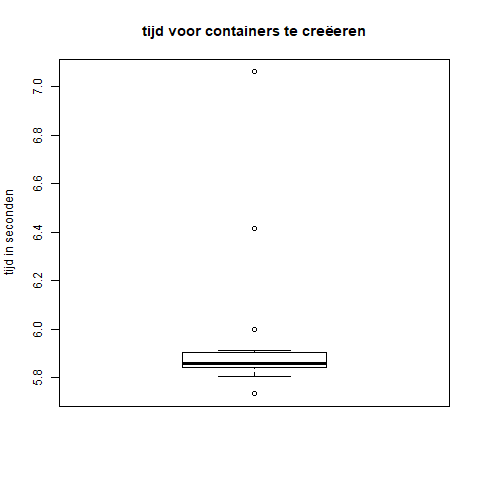
\includegraphics[scale=0.5]{img/centosboxplotprovision.png}
\end{center}

%% boxplot
\begin{center}
	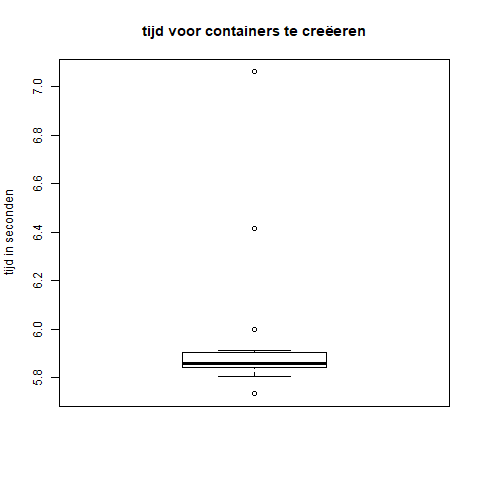
\includegraphics[scale=0.5]{img/centosboxplotprovision.png}
\end{center}

%% gemiddelde
$\mu = 5.972333$

%% variantie
$\sigma^2 = 0.1150491$

%% standaarddeviatie
$\sigma = 0.3391889$

De installatie van de Windows opstelling duurde gemiddeld 10 keer langer dan de centOS-opstelling. De gemiddelde tijd voor een volledige installatie was immers 45 minuten. De variantie en standaarddeviatie lagen ook . Hier waren verschillende redenen voor:

\begin{itemize}[noitemsep]
	\item Installatie Windows OS
\end{itemize}

Om te beginnen duurde de installatie van het besturingssysteem langer omdat er een GUI gebruikt werd. Als Windows Server Core werd gebruikt zou de performantie al sterk verbeteren. Maar, dan kon men geen Docker CE for Windows installeren. Windows Server Nano was helaas ook geen optie, omdat deze helemaal niet ondersteund werd door Docker for Windows, zelfs niet voor Docker EE. Ten slotte hoefde CentOS ook niet heropgestart te worden na de installatie van Docker.

\begin{itemize}[noitemsep]
	\item Microsoft SQL server container
\end{itemize}

De MSSQL server container voor Windows was meer dan 10 keer zo groot als de Linux variant,  6GBs tegenover 479MBs. Hierdoor was de installatie een groot deel van zijn tijd bezig met het downloaden van deze Docker Image.

\subsection{Performantie applicatie}
Ten slotte kan men hieronder ook de resultaten zien van 'time vagrant provision' voor de Windows-opstelling van alleen de benodigde tijd om de containers te installeren.

%% plot
\begin{center}
	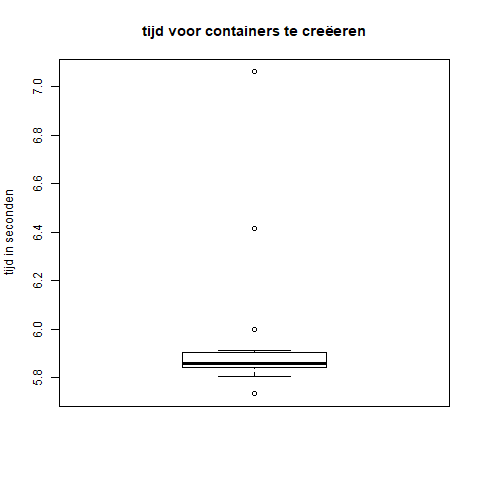
\includegraphics[scale=0.5]{img/centosboxplotprovision.png}
\end{center}

%% boxplot
\begin{center}
	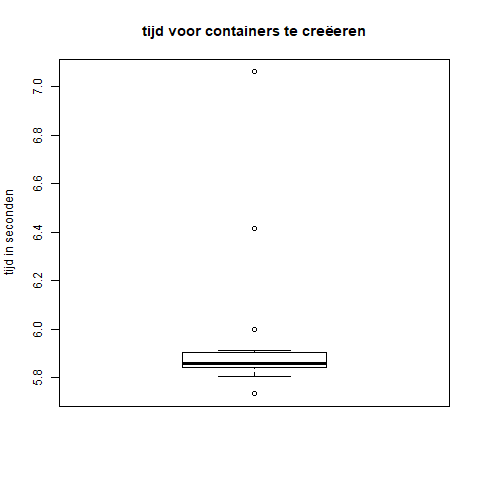
\includegraphics[scale=0.5]{img/centosboxplotprovision.png}
\end{center}

%% gemiddelde
$\mu = 5.972333$

%% variantie
$\sigma^2 = 0.1150491$

%% standaarddeviatie
$\sigma = 0.3391889$

Hier waren de resultaten al iets meer gelijk aan de CentOS-opstelling. Doordat de Windows-opstelling nu niet meer tijd verloor met het installeren van een GUI, heropstarten of downloaden van grotere Docker Images.

\section{Conclusie}
